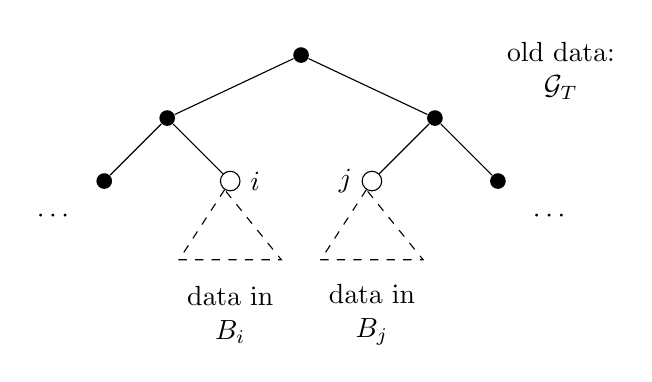
\begin{tikzpicture}[x=1cm,y=1cm,
 old/.style={circle,fill=black,inner sep=2pt},
 fresh/.style={circle,draw,fill=white,inner sep=2.5pt}]
 \node[old,label=above:{$\varnothing$}] (r) at (0,1.6) {};
 \node[old] (a) at (-1.7,.8) {};
 \node[old] (b) at (1.7,.8) {};
 \node[old] (a1) at (-2.5,0) {};
 \node[fresh,label=right:{$i$}] (i) at (-.9,0) {};
 \node[fresh,label=left:{$j$}] (j) at (.9,0) {};
 \node[old] (b1) at (2.5,0) {};
 \draw (r)--(a)--(a1) (a)--(i) (r)--(b)--(j) (b)--(b1);
 \draw[dashed] (i)--(-1.55,-1)--(-.25,-1)--cycle;
 \draw[dashed] (j)--(.25,-1)--(1.55,-1)--cycle;
 \node[align=center] at (-.9,-1.7) {data in\\$B_i$};
 \node[align=center] at (.9,-1.7) {data in\\$B_j$};
 \node[align=center] at (3.3,1.4) {old data:\\$\mathcal G_T$};
 \node at (-3.15,-.45) {$\cdots$};
 \node at (3.15,-.45) {$\cdots$};
\end{tikzpicture}
